\documentclass{minimal}
\usepackage{bm}
\usepackage{epsfig,color}
\usepackage[papersize={576.00bp,432.00bp},text={576.00bp,432.00bp}]{geometry}
\begin{document}
\centering
% Title: glps_renderer figure
% Creator: GL2PS 1.3.8, (C) 1999-2012 C. Geuzaine
% For: Octave
% CreationDate: Mon Aug 31 11:31:09 2015
\setlength{\unitlength}{1pt}
\begin{picture}(0,0)
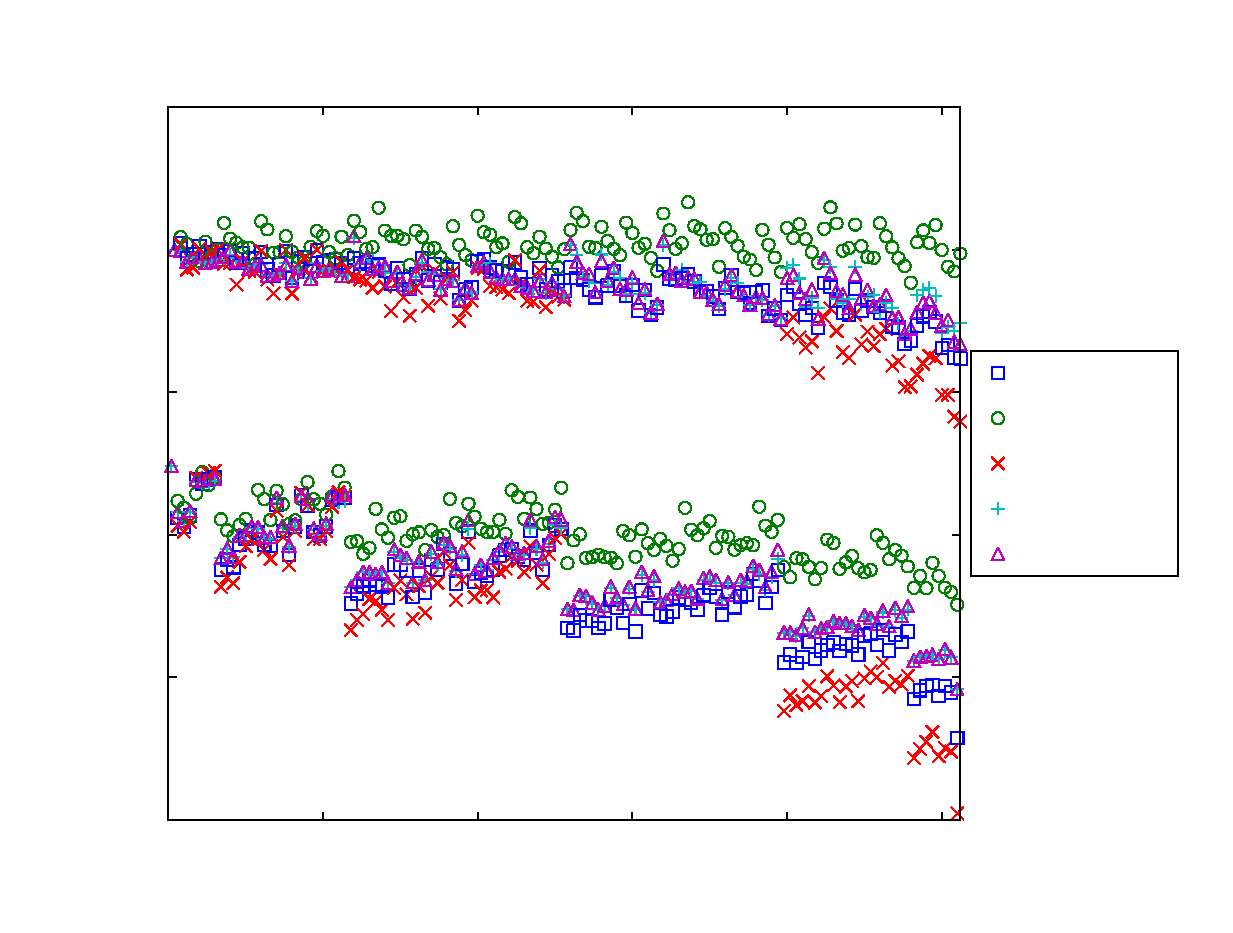
\includegraphics{normalized_energy_new-inc}
\end{picture}%
\begin{picture}(576,432)(0,0)
\fontsize{16}{0}
\selectfont\put(72.7998,41.1958){\makebox(0,0)[t]{\textcolor[rgb]{0,0,0}{{0}}}}
\fontsize{16}{0}
\selectfont\put(147.05,41.1958){\makebox(0,0)[t]{\textcolor[rgb]{0,0,0}{{50}}}}
\fontsize{16}{0}
\selectfont\put(221.3,41.1958){\makebox(0,0)[t]{\textcolor[rgb]{0,0,0}{{100}}}}
\fontsize{16}{0}
\selectfont\put(295.551,41.1958){\makebox(0,0)[t]{\textcolor[rgb]{0,0,0}{{150}}}}
\fontsize{16}{0}
\selectfont\put(369.801,41.1958){\makebox(0,0)[t]{\textcolor[rgb]{0,0,0}{{200}}}}
\fontsize{16}{0}
\selectfont\put(444.051,41.1958){\makebox(0,0)[t]{\textcolor[rgb]{0,0,0}{{250}}}}
\fontsize{16}{0}
\selectfont\put(67.7979,46.2002){\makebox(0,0)[r]{\textcolor[rgb]{0,0,0}{{-20}}}}
\fontsize{16}{0}
\selectfont\put(67.7979,114.66){\makebox(0,0)[r]{\textcolor[rgb]{0,0,0}{{-15}}}}
\fontsize{16}{0}
\selectfont\put(67.7979,183.12){\makebox(0,0)[r]{\textcolor[rgb]{0,0,0}{{-10}}}}
\fontsize{16}{0}
\selectfont\put(67.7979,251.58){\makebox(0,0)[r]{\textcolor[rgb]{0,0,0}{{-5}}}}
\fontsize{16}{0}
\selectfont\put(67.7979,320.04){\makebox(0,0)[r]{\textcolor[rgb]{0,0,0}{{0}}}}
\fontsize{16}{0}
\selectfont\put(67.7979,388.5){\makebox(0,0)[r]{\textcolor[rgb]{0,0,0}{{5}}}}
\fontsize{16}{0}
\selectfont\put(262.881,28.1958){\makebox(0,0)[t]{\textcolor[rgb]{0,0,0}{{\textbf{cluster}}}}}
\fontsize{16}{0}
\selectfont\put(47.7979,217.35){\rotatebox{90}{\makebox(0,0)[b]{\textcolor[rgb]{0,0,0}{{\textbf{normalized energy [eV]}}}}}}
\fontsize{16}{0}
\selectfont\put(483.661,260.689){\makebox(0,0)[l]{\textcolor[rgb]{0,0,0}{{Gaussian}}}}
\fontsize{16}{0}
\selectfont\put(483.661,239.02){\makebox(0,0)[l]{\textcolor[rgb]{0,0,0}{{abinit}}}}
\fontsize{16}{0}
\selectfont\put(483.661,217.35){\makebox(0,0)[l]{\textcolor[rgb]{0,0,0}{{nwchem}}}}
\fontsize{16}{0}
\selectfont\put(483.661,195.681){\makebox(0,0)[l]{\textcolor[rgb]{0,0,0}{{NN (I)}}}}
\fontsize{16}{0}
\selectfont\put(483.661,174.011){\makebox(0,0)[l]{\textcolor[rgb]{0,0,0}{{NN(II)}}}}
\end{picture}
\end{document}
